Success in calculus depends on your background in algebra, trigonometry, 
analytic geometry and functions. In this chapter, we review many of the
concepts you will need to be familiar with in order to succeed in this course.

\section{Algebra}\label{sec:Algebra}

% Input each subsection
%%%%%%%%%%%%%%%%%%%%%%%%%%%%%%%%%%%%%%%%%%%%%%%%%%%%%%%%%%%%%%%%%%%%%%%
\subsection{Sets and Number Systems}

A \dfont{set} can be thought of as any collection of \ifont{distinct} objects, called {\bf{elements}} of the set.\\

In general, there are three ways to describe sets.  

	
\begin{formulabox}[Ways to Describe Sets]
	
	\begin{enumerate}
		
		\item \textbf{Verbally:} Use a sentence to define a set.\index{set ! verbal description}
		
		\item \textbf{Roster Notation:}  Begin with a left brace `$\{$', list each element of the set \textit{only once} and then end with a right brace `$\}$'.\index{set ! roster method}
		
		\item \textbf{Set-Builder Notation:} A combination of verbal and roster notation using a ``dummy variable'' such as $x$.\index{set ! set-builder notation}\index{set-builder notation}
	\end{enumerate}
\end{formulabox} 	


\begin{example}{Roster Notation for Sets}{Sets}
	The collection $\{a,b,1,2\}$ is a set. It consists of the collection of
	four distinct objects, namely, $a$, $b$, $1$ and $2$. The order of the elements doesn't matter, so the same set could be described as $\{2,a,1,b\}$. 
\end{example}

Typically, sets are represented using 
\dfont{set-builder notation} and are surrounded by braces.
Recall that $(,)$ are called \dfont{parentheses} or \dfont{round brackets};
$[,]$ are called \dfont{square brackets}; and $\{,\}$ are called \dfont{braces} or \dfont{curly brackets}. \\

\begin{example}{Set-Builder Notation for Sets}{SetBuilder}
The expression $\displaystyle{ \{x \, \ssep  x \geq 0 \} }$ can be read as the set of all elements $x$ such that $x$ is greater than or equal to zero.  The vertical bar $\ssep$, which can also be written as a colon $:$, is a separator that can be read as "such that", "for which", or "with the property that". 
\end{example}	

Let $S$ be any set. We use the notation $\dfont{x\in S}$ to mean that $x$ 
is an element \ifont{inside} of the set $S$, and the notation $\dfont{x\not\in S}$ to mean that $x$ is \ifont{not} an element of the set $S$. \\


\begin{example}{Set Membership}{SetMembership}
If $S=\{a,b,c\}$, then $a\in S$ but $d\not\in S$.
\end{example}

%The \dfont{intersection} between two sets $S$ and $T$ is denoted 
%by $S\cap T$ and is the collection of all elements that belong to 
%\ifont{both} $S$ and $T$. The \dfont{union} between two sets $S$ 
%and $T$ is denoted by $S\cup T$ and is the collection of all elements 
%that belong to \ifont{either} $S$ or $T$ (or both). \\
%
%\begin{example}{Union and Intersection}{UnionIntersection}
%Let $S=\{a,b,c\}$ and $T=\{b,d\}$.
%Then $S\cap T=\{b\}$ and $S\cup T=\{a,b,c,d\}$. 
%Note that we do \ifont{not} write the element $b$ twice in $S\cup T$ even 
%though $b$ is in both $S$ and $T$.
%\end{example}

Numbers can be classified into sets called \dfont{number systems}.


\begin{formulabox}[Sets of Numbers]

\begin{enumerate}
	
	\item The \textbf{Empty Set}:\index{set ! empty}\index{empty set} $\emptyset=\{ \}=\{x\,|\,\mbox{$x
		\neq x$}\}$.  This is the set with no elements.  Like the number `$0$,' it  plays a vital role in mathematics.
	
	\item The \textbf{Natural Numbers}:\index{natural number ! set of}\index{natural number ! definition of} $\mathbb N= \{ 1, 2, 3,  \ldots\}$ The periods of ellipsis here indicate that the natural numbers contain $1$, $2$, $3$, `and so forth'.
	
	\item The \textbf{Whole Numbers}:\index{whole number ! set of}\index{whole number ! definition of} $\mathbb W = \{ 0, 1, 2, \ldots \}$
	
	\item The \textbf{Integers}:\index{integer ! set of}\index{integer ! definition of} $\mathbb Z=\{ \ldots, -1, -2, -1, 0, 1, 2, 3, \ldots \}$
	
	\item The \textbf{Rational Numbers}:\index{rational number ! set of}\index{rational number ! definition of} $\mathbb Q=\left\{\frac{a}{b} \, | \, a \in \mathbb Z \, \mbox{and} \, b \in \mathbb Z \right\}$.  \underline{Ratio}nal numbers are the \underline{ratio}s of integers (provided the denominator is not zero!)  It turns out that another way to describe the rational numbers is: \[\mathbb Q=\{x\,|\,\mbox{$x$ possesses a repeating or terminating decimal representation.}\}\]
	
	\item The \textbf{Real Numbers}:\index{real number ! set of}\index{real number ! definition of} $\mathbb R = \{ x\,|\,\mbox{$x$ possesses a decimal representation.}\}$
	
	\item The \textbf{Irrational Numbers}:\index{irrational number ! set of}\index{irrational number ! definition of} $\mathbb P = \{x\,|\,\mbox{$x$ is a non-rational real number.}\}$  Said another way, an \underline{ir}rational number is a decimal which neither repeats nor terminates.
	
	\item The \textbf{Complex Numbers}:\index{complex number ! set of}\index{complex number ! definition of} $\mathbb C=\{a+bi\,|\,\mbox{$a$,$b \in \mathbb R$ and $i=\sqrt{-1}$}\}$  Despite their importance, the complex numbers play only a minor role in the text.
	
\end{enumerate}
\end{formulabox}

It is important to note that every natural number is a whole number, which, in turn, is an integer.   Each integer is a rational number (take $b =1$ in the above definition for $\mathbb Q$) and the rational numbers are all real numbers, since they possess decimal representations.   If we take $b=0$ in the above definition of $\mathbb C$, we see that every real number is a complex number.  In this sense, the sets $\mathbb N$, $\mathbb W$, $\mathbb Z$, $\mathbb Q$, $\mathbb R$, and $\mathbb C$ are nested.



%\begin{center}
%  \begin{tabular}{| c || c | c |}
%    \hline
%    $\mathbb{N}$ & the \dfont{natural} numbers 
%    		& $\{1, 2, 3,\ldots\}$ \\ \hline
%    $\mathbb{Z}$ & the \dfont{integers} 
%    		& $\{\dots,-3,-2, -1, 0, 1, 2, 3,\dots\}$ \\ \hline
%    $\mathbb{Q}$ & the \dfont{rational} numbers 
%    		& Ratios of integers: $\left\{\frac{p}{q}\, \ssep\,p,q\in\mathbb{Z},q\not=0\right\}$ \\ \hline
%    $\mathbb{R}$ & the \dfont{real} numbers 
%    		& Can be written using a finite or infinite \ifont{decimal expansion} \\ \hline
%    $\mathbb{C}$ & the \dfont{complex} numbers 
%    		& These allow us to solve equations such as $x^2+1=0$ \\
%    \hline
%  \end{tabular}
%\end{center}

%In the table, the set of rational numbers is written using
%set-builder notation. The vertical bar $\ssep$, which can also be written as a colon $:$, is a separator that can be read as "such that", "for which", or "with the property that". 
%The expression $\left\{\frac{p}{q}\, \ssep\,p,q\in\mathbb{Z},q\not=0\right\}$ can be read out loud as
%\ifont{the set of all fractions $p$ over $q$ such that $p$ and $q$ are both integers and $q$ is not equal to zero}. 
%\\

\begin{example}{Rational Numbers}{RationalNumbers}
The numbers $-\frac{3}{4}$, $2.647$, $17$, $0.\bar{7}$ are all rational numbers. 
You can think of rational numbers as \ifont{fractions} of one integer over another. 
Note that 2.647 can be written as a fraction: 
\[ 2.647=2.647\times\frac{1000}{1000}=\frac{2647}{1000} \]
Also note that in the expression $0.\bar{7}$, the bar over the $7$ indicates 
that the $7$ is repeated forever: 
\[ 0.77777777\ldots=\frac{7}{9}\]
\vspace{-0.5cm}
\end{example} 

All rational numbers are real numbers with the property that
their decimal expansion either \ifont{terminates} after a finite number 
of digits or begins to \ifont{repeat} the same finite sequence of digits over and over.
Real numbers that are not rational are called \dfont{irrational}. \\



\begin{example}{Irrational Numbers}{IrrationalNumbers}
Some of the most common irrational numbers include:
\begin{itemize}
	\item $\sqrt 2$.\quad 
			Can you prove this is irrational? (The proof uses a technique called \ifont{contradiction}.)
	\item $\pi$.\quad 
			Recall that $\pi$ (\dfont{pi}) is defined as the ratio of the circumference of a circle to its diameter and can be approximated by $3.14159265$.
	\item $e$.\quad 
			Sometimes called Euler's number, $e$ can be approximated by $2.718281828459$. 
			We will review the definition of $e$ in a later chapter.
\end{itemize}
\end{example}

Let $S$ and $T$ be two sets. If every element of $S$ is also an element of $T$, then
we say $S$ is a \dfont{subset} of $T$ and write $S\subseteq T$. Furthermore, if $S$ is
a subset of $T$ but not equal to $T$, we often write $S\subset T$.
The five sets of numbers in the table give an increasing sequence of sets:
\[ \mathbb{N} \subset \mathbb{Z} \subset \mathbb{Q} \subset \mathbb{R} \subset \mathbb{C}. \]

That is, all natural numbers are also integers, all integers are also rational numbers, all rational numbers are also real numbers, and all real numbers are also complex numbers.\\

For the most part, this textbook focuses on sets whose elements come from the real numbers $\mathbb R$.  Recall that we may visualize $\mathbb R$ as a line. Segments of this line are called \textbf{intervals}\index{interval ! definition of} of numbers. Below is a summary of the so-called \textbf{interval notation}\index{interval ! notation for} associated with given sets of numbers.  For intervals with finite endpoints, we list the left endpoint, then the right endpoint.  We use square brackets, `$[$' or `$]$', if the endpoint is included in the interval and use a filled-in or `closed' dot to indicate membership in the interval. Otherwise, we use parentheses, `$($' or `$)$' and an `open' circle to indicate that the endpoint is not part of the set.  If the interval does not have finite endpoints, we use the symbols $-\infty$ to indicate that the interval extends indefinitely to the left and $\infty$ to indicate that the interval extends indefinitely to the right.  Since infinity is a concept, and not a number, we always use parentheses when using these symbols in interval notation, and use an appropriate arrow to indicate that the interval extends indefinitely in one (or both) directions.\\




\subsection{Inequalities, Intervals and Solving Basic Inequalities}\label{subsec:IneqInterval}

\subsection*{Inequality Notation}
Recall that we use the symbols $<,>,\leq,\geq$ when writing an inequality.
In particular,
\begin{itemize}
	\item $a<b$ means $a$ is to the \ifont{left} of $b$ (that is, 
				$a$ is \ifont{strictly less} than $b$),
	\item $a\leq b$ means $a$ is to the \ifont{left of or the same} 
				as $b$ (that is, $a$ is \ifont{less than or equal} to $b$),
	\item $a>b$ means $a$ is to the \ifont{right} of $b$ (that is, $a$ 
				is \ifont{strictly greater} than $b$),
	\item $a\geq b$ means $a$ is to the \ifont{right of or the same} 
				as $b$ (that is, $a$ is \ifont{greater than or equal} to $b$).
\end{itemize}

\noindent To keep track of the difference between the symbols, some students use the following mnemonic.\\

\begin{formulabox}[Mnemonic]
The $<$ symbol looks like a slanted \ifont{L} which stands for ``\ifont{L}ess than''.
\end{formulabox}

\bigskip

\begin{example}{Inequalities}{Inequalities}
The following expressions are true: 
\[ 1<2,\quad 
   -5<-2,\quad 
   1\leq 2,\quad
   1\leq 1,\quad
   4\geq\pi>3,\quad
   7.23\geq -7.23.
\]
\vspace{-0.5cm}
\end{example}

The real numbers are ordered and are often illustrated using the \dfont{real number line}:
\[
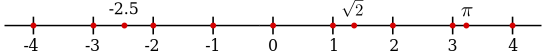
\includegraphics[width=5in]{images/real-number-line} 
\]

 
\subsection*{Intervals}
Assume $a,b$ are real numbers with $a<b$ (i.e., $a$ is strictly 
less than $b$). An \dfont{interval} is a set of every real number 
between two indicated numbers and may or may not contain the two numbers themselves.
When describing intervals we use both round brackets and square brackets.

(1) Use of round brackets in intervals: $(~,~)$.
The notation \dfont{(a,b)} is what we call the \dfont{open interval from a to b} 
and consists of all the numbers between $a$ and $b$, but does \ifont{not} include $a$ or $b$.
Using set-builder notation we write this as:
\[ (a,b)=\{x\in\mathbb{R}\, \ssep \,a<x<b\} \]
We read $\{x\in\mathbb{R}\,\ssep \,a<x<b\}$ as ``the set of real numbers $x$ such that $x$ is greater than $a$ and less than $b$''. On the real number line we represent this with the following diagram:
\[
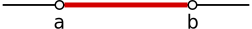
\includegraphics[width=2in]{images/interval-open} 
\]
Note that the circles on $a$ and $b$ are not shaded in, we call these \dfont{open circles} and use them to denote that $a$,$b$ are \ifont{omitted} from the set.

(2) Use of square brackets in intervals: $[~,~]$.
The notation \dfont{[a,b]} is what we call the \dfont{closed interval from a to b} 
and consists of all the numbers between $a$ and $b$ and \ifont{including} $a$ and $b$.
Using set-builder notation we write this as
\[ [a,b]=\{x\in\mathbb{R}\,|\,a\leq x\leq b\} \]
On the real number line we represent this with the following diagram:
\[
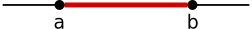
\includegraphics[width=2in]{images/interval-closed} 
\]
Note that the circles on $a$ and $b$ are shaded in, we call these \dfont{closed circles} and use them to denote that $a$ and $b$ are \ifont{included} in the set.

To keep track of when to shade a circle in, you may find the following mnemonic useful:\\

\begin{formulabox}[Mnemonic]
The round brackets $(,)$ and non-shaded circle both form an ``O'' shape which stands for ``Open and Omit''.
\end{formulabox}

Taking combinations of round and square brackets, we can write different 
possible types of intervals. 


%%%%%%%%%%%%%%%%%%%%%%%%%%%%%%%%%%%%%
%%%%%%%%%%%%%%%%%%%%%%%%%%%%%%%%%%%
\begin{formulabox}[Interval Notation]

Let $a$ and $b$ be real numbers with $a<b$.\\

\vspace{2mm}
	\begin{tabular}{|c|c|c|} \hline
		&& \\ [-1em]
		Set of Real Numbers & Interval Notation &  Region on the Real Number Line  \\
		\hline
		
		&  & \\
		\shortstack{$\{x\,\ssep \,a<x<b\}$ \\ \hfill}& \shortstack{$(a,b)$ \\ \hfill} & 
		
		  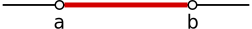
\includegraphics[width=1.8in]{images/interval-open}  \\ \hline
		
		& &  \\
		\shortstack{$\{x\,\ssep \,a\leq x<b\}$ \\ \hfill}& \shortstack{$[a,b)$ \\ \hfill} & 
		
		 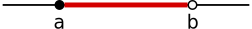
\includegraphics[width=1.8in]{images/interval-1} \\
		\hline
		
		&  & \\
		\shortstack{$\{x\,\ssep \,a<x\leq b\}$ \\ \hfill}&\shortstack{$(a,b]$ \\ \hfill} & 
		
		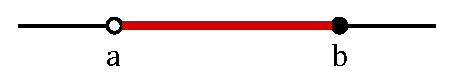
\includegraphics[width=1.8in]{images/interval-2} \\
		\hline
		
		&  & \\
		\shortstack{$\{x\,\ssep \,a\leq x \leq b\}$ \\ \hfill}& \shortstack{$[a,b]$ \\ \hfill}& 
		
		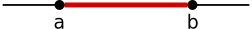
\includegraphics[width=1.8in]{images/interval-closed} \\
		\hline
		
		& & \\
		\shortstack{$\{x\, \ssep \, x<b\}$ \\ \hfill}& \shortstack{$(-\infty,b)$ \\ \hfill}& 
		
		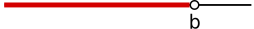
\includegraphics[width=1.8in]{images/interval-5} \\
		\hline
		
		&  & \\
		
		\shortstack{$\{x\, \ssep \, x \leq b\}$ \\ \hfill} & \shortstack{$(-\infty,b]$ \\ \hfill}& 
		
		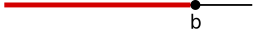
\includegraphics[width=1.8in]{images/interval-6}
		
		  \\
		\hline
		
		&  & \\
		\shortstack{$\{x\, \ssep \, x>a\}$ \\ \hfill}& \shortstack{$(a,\infty)$ \\ \hfill}& 
		
		 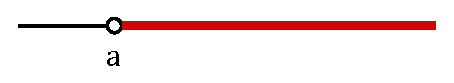
\includegraphics[width=1.8in]{images/interval-3} \\
		\hline
		
		&  & \\
		\shortstack{$\{x\, \ssep \, x \geq a \}$ \\ \hfill}& \shortstack{$[a,\infty)$ \\ \hfill} & 
		
		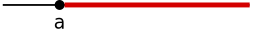
\includegraphics[width=1.8in]{images/interval-4}
		
		 \\
		\hline
		
		&  & \\
		\shortstack{$\mathbb R$ \\ \hfill}& \shortstack{$(-\infty,\infty)$ \\ \hfill} & 
		
		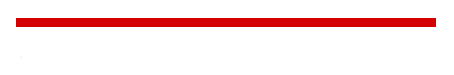
\includegraphics[width=1.8in]{images/interval-7}
		
		   \\
		\hline
		
	\end{tabular}
	
\end{formulabox}

%%%%%%%%%%%%%%%%%%%%%%%%%%%%%%%%
%%%%%%%%%%%%%%%%%%%%%%%%%%%%%

%\[
%\begin{array}{|c|c|c|}
%\hline
%&& \\
%(a,b)=\{x\in\mathbb{R}\,\ssep \,a<x<b\} 
%	& [a,b]=\{x\in\mathbb{R}\, \ssep \,a\leq x\leq b\} 
%	& [a,b)=\{x\in\mathbb{R}\, \ssep \,a\,\leq x<b\}\\
%	~&~&~\\
%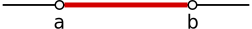
\includegraphics[width=1.8in]{images/interval-open} 
%	& 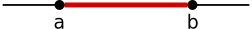
\includegraphics[width=1.8in]{images/interval-closed}
%	& 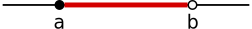
\includegraphics[width=1.8in]{images/interval-1}\\
%
%\hline
%&& \\
%(a,b]=\{x\in\mathbb{R}\, \ssep \,a<x\leq b\}
%	& (a,\infty)=\{x\in\mathbb{R}\, \ssep \,x>a\} 
%	& [a,\infty)=\{x\in\mathbb{R}\, \ssep \,x\geq a\}\\
%	~&~&~\\
%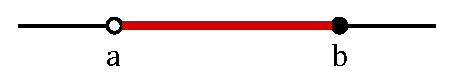
\includegraphics[width=1.8in]{images/interval-2} 
%	& 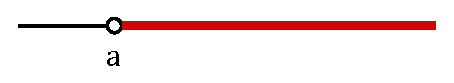
\includegraphics[width=1.8in]{images/interval-3}
%	& 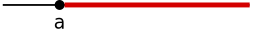
\includegraphics[width=1.8in]{images/interval-4}\\
%
%\hline
%&& \\
%(-\infty,b)=\{x\in\mathbb{R}\, \ssep \,x<b\} 
%	& (-\infty,b]=\{x\in\mathbb{R}\, \ssep \,x\leq b\}
%	& (-\infty,\infty)=\mathbb{R}=\mbox{all real numbers}\\
%	~&~&~\\
%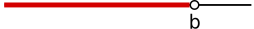
\includegraphics[width=1.8in]{images/interval-5} 
%	& 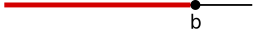
\includegraphics[width=1.8in]{images/interval-6}
%	& 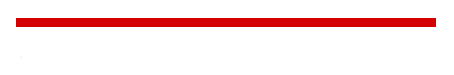
\includegraphics[width=1.8in]{images/interval-7}\\
%\hline
%\end{array}
%\]

\textit{Note}: Any set which is bound at positive and/or negative infinity is an open interval.\\

For an example, consider the sets of real numbers described below.

\begin{example}{Interval Notation}{IntervalNotation}
	\begin{tabular}{|c|c|c|} \hline
		
		Set of Real Numbers & Interval Notation &  Region on the Real Number Line  \\
		\hline
		& &  \\
		\shortstack{$\{x\, \ssep \,1\leq x< 3\}$ \\ \hfill} & \shortstack{$[1,3)$ \\ \hfill} & 
		  \includegraphics[width=2.3in]{images/interval-1ex} \\
		\hline
		
		&  & \\
		\shortstack{$\{x\, \ssep \,-1\leq x \leq 4\}$ \\ \hfill}& \shortstack{$[-1,4]$ \\ \hfill} & 
		\includegraphics[width=2.3in]{images/interval-closedex}  \\
		\hline
		
		&  & \\
		
		\shortstack{$\{x\, \ssep  \, x \leq 5 \}$ \\ \hfill} & \shortstack{$(-\infty, 5]$ \\ \hfill} &
		\includegraphics[width=2.3in]{images/interval-6ex}  \\
		\hline
		
		&  & \\
		\shortstack{$\{x\, \ssep  \, x > -2 \}$ \\ \hfill} & \shortstack{$(-2, \infty)$ \\ \hfill} &  	
	\includegraphics[width=2.3in]{images/interval-3ex}  \\
		\hline
		
	\end{tabular}
\end{example}	


We will often have occasion to combine sets.  There are two basic ways to combine sets:  \textbf{intersection}
and \textbf{union}.  We define both of these concepts below.

\begin{definition}   
	
	SSuppose $A$ and $B$ are two sets.
		
		\begin{itemize}
			
			\item The \textbf{intersection}\index{set ! intersection}\index{intersection of two sets} of $A$ and $B$:  $A \cap B = \{ x \, \ssep  \, x \in A \, \text{and} \,\, x \in B \}$
			
			\item The \textbf{union}\index{set ! union}\index{union of two sets} of $A$ and $B$: $A \cup B = \{ x \, \ssep  \, x \in A \, \text{or} \,\, x \in B \, \, \text{(or both)} \}$
			
		\end{itemize}
		
\end{definition}
	
Said differently, the intersection of two sets is the overlap of the two sets -- the elements which the sets have in common.  The union of two sets consists of the totality of the elements in each of the sets, collected together.	
	
\begin{example}{Union and Intersection}{UI1}	
If $A = \{ 1,2,3 \}$ and $B = \{2,4,6 \}$, then $A \cap B = \{2\}$ and $A \cup B = \{1,2,3,4,6\}$. 
\end{example}

\begin{example}{Union and Intersection}{UI2}
  If $A = [-5,3)$ and $B = (1, \infty)$, find $A \cap B$ and $A\cup B$.  
\end{example}
\begin{solution}
	To find $A\cap B$, we shade  the overlap of the two and obtain $A \cap B = (1,3)$. \\
	$$\includegraphics[scale=0.2]{images/interval-unionex}$$
	
	 To find $A \cup B$, we shade each of $A$ and $B$ and describe the resulting shaded region to find  $A \cup B = [-5,\infty)$.\\
	 $$\includegraphics[scale=0.2]{images/interval-unionex2}$$
	 
\end{solution}	



While both intersection and union are important, we have more occasion to use union in this text than intersection, simply because most of the sets of real numbers we will be working with are either intervals or are unions of intervals, as the following example illustrates.

%%%%%%%%%%%%%%%
%%%%%%%%%%%%
\begin{example}{Union}{union}
	
Express the following sets of numbers using interval notation.\\
	
	\begin{tabular}{lcl}
			(a) \hspace{2mm}  $\{ x \, \ssep  \, x \leq -2 \, \, \text{or} \, \,  x \geq 2 \}$
			& \hspace{2cm}
			& (b) \hspace{2mm} $\{ x \, \ssep  \, x \neq 3 \}$ \\
			&& \\ [-1em]
			(c) \hspace{2mm} $\{ x \, \ssep  \, x \neq \pm 3 \}$
			&
			&(d) \hspace{2mm} $\{ x \, \ssep  \, -1 < x \leq 3 \,\, \text{or} \,\, x = 5\}$ \\
	\end{tabular} 		
		
\end{example}	
\begin{solution} 
	
	\begin{enumerate}
		
		\item  The best way to proceed here is to graph the set of numbers on the number line and glean the answer from it.  The inequality $x \leq -2$ corresponds to the interval $(-\infty, -2]$ and the inequality $x \geq 2$ corresponds to the interval $[2, \infty)$.  Since we are looking to describe the real numbers $x$ in one of these \textit{or} the other, we have $\{ x \, | \, x \leq -2 \, \, \text{or} \, \,  x \geq 2 \} = (-\infty, -2] \cup [2, \infty)$.\\
		 $$\includegraphics[scale=0.3]{images/intervals-ex1}$$
		
		
		
		\item For the set $\{ x \, | \, x \neq 3 \}$, we shade the entire real number line except $x=3$, where we leave an open circle.  This divides the real number line into two intervals, $(-\infty, 3)$ and $(3,\infty)$.  Since the values of $x$ could be in either one of these intervals \textit{or} the other, we have that $\{ x \, | \, x \neq 3 \} = (-\infty, 3) \cup (3,\infty)$\\
		$$\includegraphics[scale=0.3]{images/intervals-ex2}$$
		
	
			
		
		\item  For the set $\{ x \, | \, x \neq \pm 3 \}$, we proceed as before and exclude both $x=3$ and $x=-3$ from our set.  This breaks the number line into \textit{three} intervals, $(-\infty, -3)$, $(-3,3)$ and $(3, \infty)$.   Since the set describes real numbers which come from the first, second \textit{or} third interval, we have $\{ x \, | \, x \neq \pm 3 \} = (-\infty, -3) \cup (-3,3) \cup (3, \infty)$.\\
		$$\includegraphics[scale=0.3]{images/intervals-ex3}$$
		
		
	
		
		\item  Graphing the set $\{ x \, | \, -1 < x \leq 3 \,\, \text{or} \,\, x = 5\}$, we get one interval, $(-1,3]$ along with a single number, or point, $\{ 5\}$.  While we \textit{could} express the latter as $[5,5]$ (Can you see why?), we choose to write our answer as $\{ x \, | \, -1 < x \leq 3 \,\, \text{or} \,\, x = 5\} = (-1,3] \cup \{ 5\}$.\\
		$$\includegraphics[scale=0.3]{images/intervals-ex4}$$
		

	\end{enumerate}
	
		
\end{solution}









%%%%%%%%%%%%%%%%%%
%%%%%%%%%%%%%%%%%%%

\subsection*{Inequality Rules}\label{sec:Inequalities}
Before solving inequalities, we start with the properties and rules of inequalities.\\

%\begin{definition}{Inequality Rules}{Inequalityrules}
\begin{formulabox}[Inequality Rules]
{\bf Add/subtract a number to both sides:}\vspace{-0.2cm}
\begin{itemize}
	\item If $a<b$, then $a+c<b+c$ and $a-c<b-c$.
\end{itemize}
{\bf Adding two inequalities of the \red{same} type:}\vspace{-0.2cm}
\begin{itemize}
	\item If $a<b$ and $c<d$, then $a+c<b+d$.\\
				\ifont{Add the left sides together, add the right sides together.}
\end{itemize}
{\bf Multiplying by a \red{positive} number:}\vspace{-0.2cm}
\begin{itemize}
	\item Let $c>0$. If $a<b$, then $c\cdot a<c\cdot b$.
\end{itemize}
{\bf Multiplying by a \red{negative}  number:}\vspace{-0.2cm}
\begin{itemize}
	\item Let $c<0$. If $a<b$, then $c\cdot a>c\cdot b$.\\
		\ifont{Note that we reversed the inequality symbol!}
\end{itemize}
\end{formulabox}
%\end{definition}

Similar rules hold for each of $\leq$, $>$ and $\geq$.


\subsection*{Solving Basic Inequalities}
We can use the inequality rules to solve some simple inequalities. \\

\begin{example}{Basic Inequality}{BasicInequality}
Find all values of $x$ satisfying
\[ 3x+1>2x-3. \]
Write your answer in both interval and set-builder notation.
Finally, draw a number line indicating your solution set.
\end{example}

\begin{solution}
Subtracting $2x$ from both sides gives $x+1>-3$.
Subtracting $1$ from both sides gives $x>-4$.
Therefore, the solution is the interval $(-4,\infty)$.
In set-builder notation the solution may be written as $\{x\in\mathbb{R}\, \ssep \,x>-4\}$.
We illustrate the solution on the number line as follows:
\[
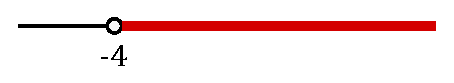
\includegraphics[width=2in]{images/ineq-ex-1}
\]
\end{solution}

Sometimes we need to split our inequality into two cases as the next example demonstrates. \\

\begin{example}{Double Inequalities}{DoubleInequalities}
Solve the inequality 
\[ 4>3x-2\geq 2x-1. \]
\vspace{-0.5cm}
\end{example}

\begin{solution}
We need both $\,\,4>3x-2\,\, $ and $\,\,3x-2\geq 2x-1\,\,$ to be true:
\[\begin{array}{rclcrcl}
	4 & > & 3x-2 & \hspace{5mm} \text{and} \hspace{5mm} & \hspace{3mm} 3x-2 & \geq & 2x-1\\
	6 & > & 3x & & x-2 & \geq & -1\\
	2 & > & x &  & x & \geq & 1\\
	x & < & 2 & & x & \geq & 1\\
\end{array}\]
Thus, we require $\,\,x\geq 1\,\,$ but also $\,\,x<2\,\,$ to be true. 
This gives all the numbers between $1$ and $2$, including $1$ but not including $2$.
That is, the solution to the inequality $\,\,4>3x-2\geq 2x-1\,\,$ is the interval $[1,2)$.
In set-builder notation this is the set $\,\,\{x\in\mathbb{R}\, \ssep \,1\leq x<2\}$.
\end{solution}

\bigskip

\begin{example}{Positive Inequality}{4x-inequality}
Solve $4x-x^2>0$.
\end{example}

\begin{solution}
We provide two methods to solve this inequality.

\bigskip
\noindent
\ifont{First method.} Factor $4x-x^2$ as $x(4-x)$.  The product of two numbers
is positive when either both are positive or both are negative, i.e., if
either $x>0$ and $4-x>0$, or else $x<0$ and $4-x<0$.  The latter alternative
is impossible, since if $x$ is negative, then $4-x$ is greater than 4, and
so cannot be negative.  As for the first alternative, the condition $4-x>0$
can be rewritten (adding $x$ to both sides) as $4>x$, so we need:
$x>0$ and $4>x$ (this is sometimes combined in the form $4>x>0$, or,
equivalently, $0<x<4$).  In interval notation, this says that the solution
is the interval $(0,4)$.

\bigskip
\noindent
\ifont{Second method.}  Write $4x-x^2$ as $-(x^2-4x)$, and then complete
the square, obtaining 
$$-\Bigl((x-2)^2-4\Bigr)=4-(x-2)^2.$$  
For this to be positive we need $(x-2)^2<4$, which means that $x-2$ must be less
than 2 and greater than $-2$:  $-2<x-2<2$.  Adding 2 to everything gives
$0<x<4$.  

\bigskip
\noindent
Both of these methods are equally correct; you may use either
in a problem of this type.
\end{solution}

We next present another method to solve more complicated looking inequalities.
In the next example we will solve a rational inequality by using 
a number line and test points. We follow the guidelines below.\\

\begin{formulabox}[Guidelines for Solving Rational Inequalities]
\begin{enumerate}\itemsep0em 
	\item Move everything to \ifont{one side} to get a $0$ on the other side.
	\item If needed, combine terms using a \ifont{common denominator}.
	\item \ifont{Factor} the numerator and denominator.
	\item Identify points where either the numerator or denominator is $0$. Such points
				are called \dfont{split points}.
	\item Draw a \ifont{number line} and indicate your split points on the number line. 
				Draw \ifont{closed/open circles} for each split point depending on 
				if that split point satisfies the inequality (division by zero is not allowed).
	\item The split points will split the number line into subintervals. For each 
				subinterval pick a \ifont{test point} and see if the expression in Step 3 
				is positive or negative. Indicate this with a $+$ or $-$ symbol on the 
				number line for that subinterval.
	\item Now write your answer in set-builder notation. Use the union symbol 
				$\cup$ if you have multiple intervals in your solution.
\end{enumerate}
\end{formulabox}

\begin{example}{Rational Inequality}{RationalInequality1}
Write the solution to the following inequality using interval notation:
\[\frac{2-x}{2+x}\geq 1.\]
\vspace{-0.5cm}
\end{example}

\begin{solution}
One method to solve this inequality is to multiply both sides by $2+x$, but because we do not know if $2+x$ is positive or negative we must split it into two cases (\ifont{Case 1:} $2+x>0$ and \ifont{Case 2:} $2+x<0$).

Instead we follow the guidelines for solving rational inequalities:
\[
\begin{array}{rcl}
\mbox{Start with original problem:}& ~ & \displaystyle{\frac{2-x}{2+x}\geq 1}\\
\\
\mbox{Move everything to one side:}& ~ & \displaystyle{\frac{2-x}{2+x}-1 \geq 0}\\
\\
\mbox{Find a common denominator:}& ~ & \displaystyle{\frac{2-x}{2+x}-\frac{2+x}{2+x} \geq 0}\\
\\
\mbox{Combine fractions:}& ~ & \displaystyle{\frac{(2-x)-(2+x)}{2+x} \geq 0}\\
\\
\mbox{Expand numerator:}& ~ & \displaystyle{\frac{2-x-2-x}{2+x} \geq 0}\\
\\
\mbox{Simplify numerator:}& ~ & \displaystyle{\frac{-2x}{2+x} \geq 0\quad(*)}\\
\end{array}
\]
Now we have the numerator and denominator in fully factored form.
The split points are $x=0$ (makes the numerator $0$) and $x=-2$ (makes the denominator $0$).
Let us draw a number line with the split points indicated on it:
\[
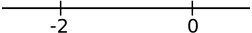
\includegraphics[width=2in]{images/ineq-rational-1}
\]
The point $x=0$ is included since if we sub $x=0$ into (*) we get $0\geq 0$ which is true.
The point $x=-2$ is not included since we cannot divide by zero.
We indicate this with open/closed circles on the number line (remember that open means omit):
\[
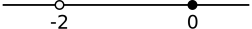
\includegraphics[width=2in]{images/ineq-rational-2}
\]
Now choosing a test point from each of the three subintervals we can determine if the expression $-2x /(2+x) $ is positive or negative.
When $x=-3$, it is negative.
When $x=-1$, it is positive.
When $x=1$, it is negative.
Indicating this on the number line gives:
\[
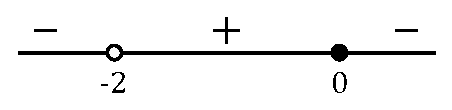
\includegraphics[width=2in]{images/ineq-rational-3}
\]
Since we wish to solve $\displaystyle{\frac{-2x}{2+x}\geq 0}$, we look at where the $+$ signs are and shade that area on the number line:
\[
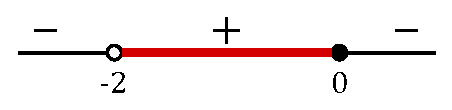
\includegraphics[width=2in]{images/ineq-rational-4}
\]
Since there is a closed circle at $0$, we include it.
Therefore, the solution is $(-2,0]$.
\end{solution}

\begin{example}{Rational Inequality}{RationalInequality2}
Write the solution to the following inequality using interval notation:
\[ \frac{2}{x+2}>{3}{x+3}. \]
\vspace{-0.5cm}
\end{example}

\begin{solution}
We provide a brief outline of the solution.
By subtracting $(3x+3)$ from both sides and using a common denominator of $x+2$,
we can collect like terms and simplify to get:
\[ \frac{-(3x^2+9x+4)}{x+2}>0. \]
The denominator is zero when $x=-2$.
Using the quadratic formula, the numerator is zero when 
$x=(-9\pm\sqrt{33})/6$ (these two numbers are approximately $-2.46$ and $-0.54$).
Since the inequality uses ``$>$'' and $0>0$ is false, 
we do not include any of the split points in our solution.
After choosing suitable test points and determining the sign of 
$-(3x^2+9x+4)/(x+2)$ we have
\[
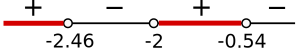
\includegraphics[width=2.5in]{images/ineq-ex-2}
\]
Looking where the $+$ symbols are located gives the solution:
$$\left(-\infty,\frac{-9-\sqrt{33}}{6}\right) \cup\left(-2,\frac{-9+\sqrt{33}}{6}\right).$$
When writing the final answer we use \ifont{exact} expressions for numbers in mathematics, not 
approximations (unless stated otherwise).
\end{solution}

\subsection{Law of Exponents}
The Law of Exponents is a set of rules for simplifying expressions that governs 
the combination of exponents (powers).
Recall that $\sqrt[n]{~}$ denotes the $n$th root. 
For example $\sqrt[3]{8}=2$ represents that the cube root of $8$ is equal to $2$.\\

\begin{definition}{Law of Exponents}{ExponentRules1}
{\bf Definitions}

If $m,n$ are positive integers, then:
\begin{multicols}{2}
\begin{enumerate}
	\item $x^n=x\cdot x\cdot\ldots\cdot x$ ($n$ times).
	\item $x^0=1$, for $x\neq 0$.
	\item $\ds{x^{-n}=\frac{1}{x^n}}$, for $x\neq 0$.
	\item $x^{m/n}=\sqrt[n]{x^m}$ or $\left(\sqrt[n]{x}\right)^m$, for $x\geq 0$.
\end{enumerate}
\end{multicols}

{\bf Combining}
\begin{multicols}{3}
\begin{enumerate}
	\item $x^ax^b=x^{a+b}$.
	\item $\ds{\frac{x^a}{x^b}=x^{a-b}}$, for $x\neq 0$.
	\item $\left(x^a\right)^b=x^{ab}=x^{ba}=\left(x^b\right)^a$.
\end{enumerate}
\end{multicols}

{\bf Distributing}
\begin{multicols}{2}
\begin{enumerate}
	\item $(xy)^a=x^ay^a$, for $x\geq 0$, $y\geq 0$.
	\item $\ds{\left(\frac{x}{y}\right)^a=\frac{x^a}{y^a}}$, for $x\geq 0$, $y>0$.
\end{enumerate}
\end{multicols}
\end{definition}

In the next example, the word \ifont{simplify} means \ifont{to make simpler} or to write the expression more compactly.\\

\begin{example}{Laws of Exponents}{LawsExponents}\label{LawsExponents}
Simplify the following expression as much as possible assuming $x,y>0$:
$$\frac{3x^{-2}y^3x}{y^2\sqrt x}.$$
\vspace{-0.5cm}
\end{example}

\begin{solution}
Using the Law of Exponents, we have:
$$\def\arraystretch{2.5}
\begin{array}{>{\displaystyle}r>{\displaystyle}c>{\displaystyle}l>{\displaystyle}l}
\frac{3x^{-2}y^3x}{y^2\sqrt x} & = & \frac{3x^{-2}y^3x}{y^2x^{\frac{1}{2}}}, 
		&\mbox{since $\ds\sqrt x = x^{\frac{1}{2}}$},\\
~ & = & \frac{3x^{-2}yx}{x^{\frac{1}{2}}}, 
		&\mbox{since $\ds\frac{y^3}{y^2}=y$},\\
~ & = & \frac{3y}{x^{\frac{3}{2}}}, 
		&\mbox{since $\ds\frac{x^{-2}x}{x^{\frac{1}{2}}}=\frac{x^{-1}}{x^{\frac{1}{2}}} =x^{-\frac{3}{2}}=\frac{1}{x^{\frac{3}{2}}}$},\\
~ & = & \frac{3y}{\sqrt{x^3}}, 
		&\mbox{since $\ds x^{\frac{3}{2}}=\sqrt{x^3}$}.
\end{array}$$
An answer of $3yx^{-3/2}$ is equally acceptable, and such an expression may prove to be computationally simpler, although a positive exponent may be preferred.
\end{solution}

\subsection{The Quadratic Formula and Completing the Square}
The technique of \dfont{completing the square} allows us to solve quadratic equations and also to determine the center of a circle/ellipse or the vertex of a parabola.

The main idea behind completing the square is to turn:
$$ ax^2 + bx + c$$
into
$$a(x - h)^2 + k.$$
One way to complete the square is to use the following formula:
$$ax^2+bx+c=a\left(x+\frac{b}{2a}\right)^2-\frac{b^2}{4a^2}+c.$$
But this formula is a bit complicated, so some students prefer following the steps outlined in the next example. \\

\begin{example}{Completing the Square}{CompletingSquare}
Solve $2x^2+12x-32=0$ by completing the square.
\end{example}

\begin{solution}
In this instance, we will \ifont{not} divide by $2$ first (usually you would) in order to demonstrate what you should do when the `$a$' value is not $1$.

\bigskip

\begin{tabular}{rl}
$2x^2+12x-32=0$ & Start with original equation.\\
\\
$2x^2+12x=32$ & Move the number over to the other side.\\
\\
$2(x^2+6x)=32$ & Factor out the $a$ from the $ax^2+bx$ expression.\\
\\
$6~~\to~~\frac{6}{2}=3~~\to~~3^2=\dfont{9}$ & Take the number in front of $x$, \\
	&  \dfont{divide by $2$}, \\
	&  then \dfont{square} it.\\
\\
$\ifont{2}(x^2+6x+\dfont{9})=32+\ifont{2}\cdot\dfont{9}$ & Add the result to both sides, \\
	&  taking $a=2$ into account.\\
\\
$2(x+3)^2=50$ & Factor the resulting perfect square trinomial.\\
\\
~ & \ifont{You have now completed the square!}\\
\\
$(x+3)^2=25~~\to~~x=2 \mbox{ or } x=-8$ & To solve for $x$, simply divide by $a=2$ \\
	& and take square roots.\\
\end{tabular}
\end{solution}

Suppose we want to solve for $x$ in the quadratic
equation $ax^2+bx+c=0$, where $a\neq 0$.
The solution(s) to this equation are given by the \dfont{quadratic formula}.\\

\begin{theorem}{The Quadratic Formula}{Quadratic Formula}
\label{QuadForm}	 
The solutions to $ax^2+bx+c=0$ (with $a\neq 0$) are $\ds{x=\frac{-b\pm\sqrt{b^2-4ac}}{2a}}$.
\end{theorem}

\begin{proof}
To prove the Quadratic Formula (Theorem \ref{QuadForm} ) we use the technique of \ifont{completing 
the square}. The general technique involves taking an expression of the 
form $x^2+rx$ and trying to find a number we can add so that we end up 
with a perfect square (that is, $(x+n)^2$). It turns out if you add $(r/2)^2$ 
then you can factor it as a perfect square.

For example, suppose we want to solve for $x$ in the equation $ax^2+bx+c=0$, where $a\neq 0$.
Then we can move $c$ to the other side and divide by $a$ (remember, $a\neq 0$ so we can divide by it) to get
$$x^2+\frac{b}{a}x=-\frac{c}{a}.$$
To write the left side as a perfect square we use what was mentioned previously.
We have $r=(b/a)$ in this case, so we must add $(r/2)^2=(b/2a)^2$ to both sides
$$x^2+\frac{b}{a}x+\left(\frac{b}{2a}\right)^2=-\frac{c}{a}+\left(\frac{b}{2a}\right)^2.$$
We know that the left side can be factored as a perfect square
$$\left(x+\frac{b}{2a}\right)^2=-\frac{c}{a}+\left(\frac{b}{2a}\right)^2.$$
The right side simplifies by using the exponent rules and finding a common denominator
$$\left(x+\frac{b}{2a}\right)^2=\frac{-4ac+b^2}{4a^2}.$$
Taking the square root we get
$$x+\frac{b}{2a}=\pm\sqrt{\frac{-4ac+b^2}{4a^2}},$$
which can be rearranged as
$$x=\frac{-b\pm\sqrt{b^2-4ac}}{2a}.$$
In essence, the quadratic formula is just completing the square.
\end{proof}
\subsection{The Absolute Value}

\begin{definition}{Absolute Value}{Absolute Value}
	\label{def:AbsoluteValue}
The \dfont{absolute value} of a number $x$ is written as $|x|$ and represents 
the \ifont{distance} $x$ is from zero. Mathematically, we define it as follows:
$$|x|=\left\{\begin{array}{cl}
x, & \mbox{if $x\geq 0$,}\\
-x, & \mbox{if $x<0$.}\\
\end{array}\right.$$
\end{definition}

Thus, if $x$ is a negative real number, then $-x$ is a positive real number.
The absolute value does \ifont{not} just turn minuses into pluses.
That is, $|2x-1|\neq 2x+1$.
You should be familiar with the following properties.\\

\begin{formulabox}[Absolute Value Properties]
\begin{enumerate}
	\item $|x|\geq 0$.
	\item $|xy|=|x||y|$.
	\item $\displaystyle{\left|\frac{1}{x} \right|=\frac{1}{|x|} }$ \hspace{2mm} when $x\neq 0$.
	\item $|-x|=|x|$.
	\item $|x+y|\leq |x|+|y|$. This is called the \dfont{triangle inequality}.
	\item $\sqrt{x^2}=|x|$.
\end{enumerate}
\end{formulabox}

\begin{example}{$\sqrt{x^2}=|x|$}{sqrtabs}
Observe that $\sqrt{(-3)^2}$ gives an answer of $3$, not $-3$.
\end{example}

When solving inequalities with absolute values, the following are helpful. %(here $a>0$ is a positive number):
%\begin{itemize}
%	\item $|x|=a$ means $x=\pm a$.
%	\item $|x|\leq a$ means $x\geq -a$ \ifont{and} $x\leq a$  (that is, $-a\leq x\leq a$).
%	\item $|x|\geq a$ means $x\leq -a$ \ifont{or} $x\geq a$.
%\end{itemize}
%
%In the above, we do require $a>0$, otherwise we end up with false expressions.
%For example, $|x|=-1$ has no solutions because $|x|$ is always positive (or zero), 
%so it will never equal $-1$. On the other hand, $|x|=1$ has the solutions $x=\pm 1$.
 
\medskip
{\bf Case 1: $a>0$.}\vspace{-0.1cm}
\begin{itemize}\setlength{\itemsep}{0 in}
\item $|x|=a$ has solutions $x=\pm a$. 
\item $|x|\leq a$ means $x\geq -a$ {\bf and} $x\leq a$  (that is, $-a\leq x\leq a$). 
\item $|x|<a$ means $x< -a$ {\bf and} $x< a$  (that is, $-a< x< a$). 
\item $|x|\geq a$ means $x\leq -a$ {\bf or} $x\geq a$. 
\item $|x|> a$ means $x< -a$ {\bf or} $x> a$. 
\end{itemize}

{\bf Case 2: $a<0$.}\vspace{-0.1cm}
\begin{itemize}\setlength{\itemsep}{0 in}
\item $|x|=a$ has no solutions. 
\item Both $|x|\leq a$ and $|x|<a$ have no solutions. 
\item Both $|x|\geq a$ and $|x|>a$ have solution set $\{x|x\in\R\}$. 
\end{itemize}

{\bf Case 3: $a=0$.}\vspace{-0.1cm}
\begin{itemize}\setlength{\itemsep}{0 in}
\item $|x|=0$ has solution $x=0$. 
\item $|x|<0$ has no solutions. 
\item $|x|\leq 0$ has solution $x=0$. 
\item $|x|>0$ has solution set $\{x\in\R|x\neq 0\}$. 
\item $|x|\geq 0$ has solution set $\{x|x\in\R\}$.
\end{itemize}
\subsection{Solving Inequalities that Contain Absolute Values}
We start by solving an equality that contains an absolute value.
To do so, we recall that if $a\geq 0$ then the solution to 
$|x|=a$ is $x=\pm a$. In cases where we are not sure if the right 
side is positive or negative, we must perform a check at the end. \\

\begin{example}{Absolute Value Equality}{AbsoluteValueEquality}
Solve for $x$ in $|2x+3|=2-x$.
\end{example}

\begin{solution} 
This means that either:
\[\begin{array}{ccc}
	2x+3=+(2-x) & \mbox{\ifont{or}} & 2x+3=-(2-x)\\
	2x+3=2-x & \mbox{\ifont{or}} & 2x+3=-2+x\\
	3x=-1 & \mbox{\ifont{or}} & x=-5\\
	x=-1/3 & \mbox{\ifont{or}} & x=-5\\
\end{array}\]
Since we do not know if the right side $``a=2-x"$ is positive or negative, we must perform a check of our answers omit any that are incorrect.

If $x=-1/3$, then we have $LS=|2(-1/3)+3|=|-2/3+3|=|7/3|=7/3$ and $RS=2-(-1/3)=7/3$.
In this case $LS=RS$, so $x=-1/3$ is a solution.

If $x=-5$, then we have $LS=|2(-5)+3|=|-10+3|=|-7|=7$ and $RS=2-(-5)=2+5=7$.
In this case $LS=RS$, so $x=-5$ is a solution.
\end{solution}

We next look at absolute values and inequalities. \\

\begin{example}{Absolute Value Inequality}{AbsoluteValueInequality}
Solve $|x-5|<7$.
\end{example}

\begin{solution} 
This simply means $-7<x-5<7$.
Adding $5$ to each gives $-2<x<12$.
Therefore the solution is the interval $(-2,12)$.
\end{solution}

In some questions you must be careful when multiplying by a negative number as in the next problem. \\

\begin{example}{Absolute Value Inequality}{AbsoluteValueInequality2}
Solve $|2-z|<7$.
\end{example}

\begin{solution} 
This simply means $-7<2-z<7$.
Subtracting $2$ gives: $-9<-z<5$.
Now multiplying by $-1$ gives: $9>z>-5$. \ifont{Remember to reverse the inequality signs!}
We can rearrange this as $-5<z<9$.
Therefore the solution is the interval $(-5,9)$.
\end{solution}

\bigskip

\begin{example}{Absolute Value Inequality}{AbsoluteValueInequality3}
Solve $|2-z|\geq 7$.
\end{example}

\begin{solution} 
Recall that for $a>0$, $|x|\geq a$ means $x\leq -a$ or $x\geq a$.
Thus, either $2-z\leq -7$ \ifont{or} $2-z\geq 7$.
Either $9\leq z$ \ifont{or} $-5 \geq z$.
Either $z\geq 9$ \ifont{or} $z \leq -5$.
In interval notation, either $z$ is in $[9,\infty)$ \ifont{or} $z$ is in $(-\infty,-5]$.
All together, we get our solution to be: $(-\infty,-5]\cup [9,\infty)$.
\end{solution}

In the previous two examples the \ifont{only} difference is that one had $<$ in 
the question and the other had $\geq$. Combining the two solutions gives the 
\ifont{entire} real number line! \\

\begin{example}{Absolute Value Inequality}{AbsoluteValueInequality4}
Solve $0<|x-5|\leq 7$.
\end{example}

\begin{solution} 
We split this into two cases.

(1) For $0<|x-5|$ note that we always have that an absolute value is positive or zero (i.e., $0\leq |x-5|$ is always true).
So, for this part, we need to avoid $0=|x-5|$ from occurring. 
Thus, $x$ \ifont{cannot} be $5$, that is, $x\neq 5$.

(2) For $|x-5|\leq 7$, we have $-7\leq x-5\leq 7$.
Adding $5$ to each gives $-2\leq x\leq 12$.
Therefore the solution to $|x-5|\leq 7$ is the interval $[-2,12]$.

To combine (1) and (2) we need combine $x\neq 5$ with $x\in[-2,12]$.
Omitting $5$ from the interval $[-2,12]$ gives our solution to be: $[-2,5)\cup(5,12]$.
\end{solution}



%%%%%%%%%%%%%%%%%%%%%%%%%%%%%%%%%%%%%%%%%%%%
%%%%%%%%%%    EXERCISES    %%%%%%%%%%%%%%%%%
%%%%%%%%%%%%%%%%%%%%%%%%%%%%%%%%%%%%%%%%%%%%

\Opensolutionfile{solutions}[ex]
\section*{Exercises for \ref{sec:Algebra}}

\begin{enumialphparenastyle}

\begin{multicols}{2}
%%%%%%%%%%

\begin{ex}
Write the set using interval notation.
\begin{tabular}{lll}
(a) \hspace{2mm} 	$\{x\,|\, x \neq 5 \}$ 
&& (b) \hspace{2mm} 	$\{x\,|\, x \neq -1 \}$ \\
(c) \hspace{2mm}   $\{x\,|\, x \neq -3,\, 4 \}$
& & (d) \hspace{2mm}	$\{x\,|\, x \neq 0, \, 2 \}$ \\
(e) \hspace{2mm} $\{x\,|\, x \neq 2, \, -2 \}$
& & \\
(f) \hspace{2mm}  $\{x\,|\, x \neq 0,\, \pm 4 \}$ && \\
 (g) \hspace{2mm} $\{x\,|\, x \leq -1 \, \text{or} \, x \geq 1 \}$ &&\\
  (h) \hspace{2mm} 	$\{x\,|\, x < 3 \, \text{or} \, x \geq 2 \}$  && \\
(i) \hspace{2mm} $\{x\,|\, x \leq -3 \, \text{or} \, x > 0 \}$ && \\
 (j) \hspace{2mm}  $\{x\,|\, x \leq 5 \, \text{or} \, x = 6 \}$ && \\
(k) \hspace{2mm} $\{x\,|\, x > 2 \, \text{or} \, x = \pm 1 \}$ &&\\
\end{tabular}
\begin{sol}
\end{sol}
\end{ex}



\begin{ex}
Simplify the following expressions as much as possible assuming $x,y>0$:
\begin{enumerate}
	\item	$\ds\frac{x^3y^{-1/3}}{\sqrt[3]{y^2}x^2}$
	\item	$\ds\frac{3x^{-1/3}y^{-2}\sqrt[3]{x^4}}{\sqrt{9x}y^{-3}}$
	\item	$\ds\left(\frac{16x^2y}{x^4}\right)^{1/2}\frac{\sqrt[3]{x^2}}{2\sqrt{y}}$
\end{enumerate}
\begin{sol}
\begin{enumerate}
	\item	$\ds\frac{x}{y}$
	\item	$\sqrt{x}y$
	\item	$\ds\frac{2}{\sqrt[3]{x}}$
\end{enumerate}
\end{sol}
\end{ex}

%%%%%%%%%%
\begin{ex}
Find the constants $a,b,c$ if the expression
$$\frac{4x^{-1}y^2\sqrt[3]{x}}{2x\sqrt{y}}$$
is written in the form $ax^by^c$.
\begin{sol}
	$a=2$, $b=-\frac{5}{3}$, $c=\frac{3}{2}$. 
\end{sol}
\end{ex}

%%%%%%%%%%
\begin{ex}
Find the roots of the quadratic equation
$$x^2-2x-24=0$$
\begin{sol}
$x=-4$ and $x=6$.
\end{sol}
\end{ex}

%%%%%%%%%%
\begin{ex}
Solve the equation \\
$$\frac{x}{4x-16}-2=\frac{1}{x-3}.$$
\end{ex}

%\vfill \null
%\columnbreak

%%%%%%%%%%
\begin{ex}
Solve the following inequalities. Write your answer as a union of intervals.
\begin{multicols}{2}
\begin{enumerate}
	\item	$3x+1>6$
	\item	$0\leq 7x-1 < 1$
	\item	$\ds{\frac{x^2(x-1)}{(x+2)(x+3)^3}\leq 0}$
	\item	$x^2+1>0$
	\item	$x^2+1<0$
	\item	$x^2+1>2x$
	\item	$x^3>4x$
	\item	$x^3\geq4x^2$
	\item	$\dfrac{1}{x}>2$
	\item	$\dfrac{x}{x+2}\leq\dfrac{2}{x-1}$
\end{enumerate}
\end{multicols}
\begin{sol}
\begin{enumerate}
	\item	$(5/3,\infty)$
	\item	$[1/7,2/7]$
	\item	$(-\infty,-3)\cup(-2,1]$
	\item	$(-\infty,\infty)$
	\item	No solution
	\item	$(-\infty,1)\cup(1,\infty)$
	\item	$(-2,0)\cup(2,\infty)$
	\item	$[4,\infty)\cup\{0\}$
	\item	$(0,\frac{1}{2})$
	\item	$(-2,-1]\cup(1,4]$
\end{enumerate}
\end{sol}
\end{ex}

%%%%%%%%%%
\begin{ex}
Solve the equation $|6x+2|=1$.
\begin{sol}
$x=-\frac{1}{2}$ and $x=-\frac{1}{6}$.
\end{sol}
\end{ex}

%%%%%%%%%%
\begin{ex}
Find solutions to the following absolute value inequalities. Write your answer as a union of intervals.
\begin{multicols}{2}
\begin{enumerate}
	\item	$|x|\geq 2$
	\item	$|x-3|\leq 1$
	\item	$|2x+5|\geq 4$
	\item	$|x+2|<3x-6$
	\item	$|2x+5|+4\geq 1$
	\item	$5<|x+1|<8$
\end{enumerate}
\end{multicols}
\begin{sol}
\begin{multicols}{2}
\begin{enumerate}
	\item	$(-\infty,-2]\cup[2,\infty)$
	\item	$[2,4]$
	\item	$(-\infty,-9/2]\cup[-1/2,\infty)$
	\item	$(4,\infty)$
	\item	$(-\infty,\infty)$
	\item	$(-9,-6)\cup(4,7)$
\end{enumerate}
\end{multicols}
\end{sol}
\end{ex}

%%%%%%%%%%
\begin{ex}
Solve the equation $\sqrt{1-x}+x=1$.
\end{ex}

\end{multicols}

\end{enumialphparenastyle}